%
% Layout retirado de http://www.di.uminho.pt/~prh/curplc09.html#notas
%
\documentclass{report}
\usepackage{graphicx}
\usepackage[portuguese]{babel}
\usepackage[utf8]{inputenc}
\usepackage{hyperref}
%\usepackage[latin1]{inputenc}
%\usepackage{url}
\usepackage{color}
\usepackage{enumerate}
\usepackage{alltt}
\usepackage{fancyvrb}
\usepackage{listings}
\usepackage{amsmath}
\DefineVerbatimEnvironment{code}{Verbatim}{fontsize=\footnotesize}
%LISTING - GENERAL
\lstset{
	basicstyle=\small,
	numbers=left,
	numberstyle=\tiny,
	numbersep=5pt,
	breaklines=true,
    frame=tB,
	mathescape=true,
	escapeinside={(*@}{@*)}
	}


%\lstset{ %
%	language=Java,							% choose the language of the code
%	basicstyle=\ttfamily\footnotesize,		% the size of the fonts that are used for the code
%	keywordstyle=\bfseries,					% set the keyword style
%	%numbers=left,							% where to put the line-numbers
%	numberstyle=\scriptsize,				% the size of the fonts that are used for the line-numbers
%	stepnumber=2,							% the step between two line-numbers. If it's 1 each line
%											% will be numbered
%	numbersep=5pt,							% how far the line-numbers are from the code
%	backgroundcolor=\color{white},			% choose the background color. You must add \usepackage{color}
%	showspaces=false,						% show spaces adding particular underscores
%	showstringspaces=false,					% underline spaces within strings
%	showtabs=false,							% show tabs within strings adding particular underscores
%	frame=none,								% adds a frame around the code
%	%abovecaptionskip=-.8em,
%	%belowcaptionskip=.7em,
%	tabsize=2,								% sets default tabsize to 2 spaces
%	captionpos=b,							% sets the caption-position to bottom
%	breaklines=true,						% sets automatic line breaking
%	breakatwhitespace=false,				% sets if automatic breaks should only happen at whitespace
%	title=\lstname,							% show the filename of files included with \lstinputlisting;
%											% also try caption instead of title
%	escapeinside={\%*}{*)},					% if you want to add a comment within your code
%	morekeywords={*,...}					% if you want to add more keywords to the set
%}

\usepackage{xspace}

\parindent=0pt
\parskip=2pt

\setlength{\oddsidemargin}{-1cm}
\setlength{\textwidth}{18cm}
\setlength{\headsep}{-1cm}
\setlength{\textheight}{23cm}

%\def\darius{\textsf{Darius}\xspace}
%\def\antlr{\texttt{AnTLR}\xspace}
%\def\pe{\emph{Publicação Eletrónica}\xspace}

%\def\titulo#1{\section{#1}}
%\def\super#1{{\em Supervisor: #1}\\ }
%\def\area#1{{\em \'{A}rea: #1}\\[0.2cm]}
%\def\resumo{\underline{Resumo}:\\ }


%\input{LPgeneralDefintions}
\title{Processamento de Linguagens e Compiladores 3º ano\\ \textbf{Pré-processador para HTML}\\ TP2\\ Grupo 14}
\author{Artur Queiroz\\ A77136 \and  Rafael Fernandes\\ A78242 \and Rafaela Pinho\\ A77293 }
\date{\today}

\begin{document}

\maketitle

\begin{abstract}
Neste relatório será apresentado as ideias implementadas para criar um pré-processador de HTML através da ferramenta $Flex$. 
Também descrevemos as decisões tomadas e as dificuldades encontradas, bem como pequenos exemplos deforma que qualquer pessoa que leia este relatório perceba facilmente como funciona o nosso projeto.
\end{abstract}

\tableofcontents

\chapter{Introdução} \label{intro}
Escrever um documento em HTML trona-se muito cansativo, devido ao peso das "tags" que são inseridas para anotar o texto. Por exemplo, para colocar alguma coisa em negrito é necessário fazer:$ <b>(texto que queremos a negrito)</b>$. \\ 

Por isso existem pré-processadores de HTML que facilitam a tarefa da inserção dessas "tags", pois permitem ao utilizador usar anotações mais leves e mais simples. Depois, o pré-processador substitui a notação abreviada para a notação de HTML.\\ 

No nosso trabalho construímos um pré-processador que ajuda a simplificar a escrita do código HTML. 

%\section*{Estrutura do Relatório} \
%explicar como está organizado o documento, referindo os capítulos existentes em~\cite{Pereira201635}
%e a sua articulação explicando o conteúdo de cada um.
%No capítulo~\ref{fi} faz-se uma análise detalhada do problema proposto
%de modo a poder-se especificar  as entradas, resultados e formas de transformação.\\
%etc. \ldots\\
%No capítulo~\ref{concl} termina-se o relatório com uma síntese do que foi dito,
%as conclusões e o trabalho futuro

\chapter{Pré-Processador} \label{fi}
\section{Descrição informal do problema}\
Neste trabalho é necessário:
\begin{enumerate}[i)]
\item Criar marcas menos pesadas que são inseridas para anotar o texto.
\item Através do Flex construímos o processador. (ficheiro flex é o processador)
\item Passar um ficheiro através do processador para $HTML$.
\end{enumerate}

\section{Especificação dos requisitos}

Para este trabalho foi necessário encontrar símbolos que facilitassem a escrita ao utilizador e que não interferisse na passagem para HTML. 

  
\section{Expressões regulares} 

As expressões regulares usadas foram:

\begin{enumerate}[i)]
\item $ [bui]< | h[1-6]< $
\item $ [ou]l$$\backslash$$[$
\item $ dl$$\backslash$$\{$
\item $ .|$$\backslash$n
\item " $\backslash\backslash$ "

\end{enumerate}

\chapter{Codificação e Testes}
\section{Problemas de implementação, Decisões e Alternativas}
\subsection{Problemas de implementação}

De um modo geral, não tivemos muitos problemas de implementação. Simplesmente tivemos que alterar o símbolo para abrir e fechar as listas e os dicionários, pois da forma que implementamos o array, se elas tivessem todas o mesmo símbolo não sabíamos qual das "tags" estávamos a fechar.    


\subsection{Decisões}
Como já foi dito no capítulo 2, neste trabalho tivemos de escolher algumas marcas menos pesadas.\\ 
Para abreviar a escrita de formatação usamos: 

\begin{enumerate}[1-] 

\item Negrito: $\backslash$$b$$<texto>$ 

\item Itálico: $\backslash$$i$$<texto>$ 

\item Sublinhado: $\backslash$$u$$<texto>$ 

\item Níveis de títulos: $\backslash$$h[1-6]$$<texto>$ 

\item Listas não numeradas: $\backslash$$ul$$[item | item|... ]$ 

\item Listas numeradas: $\backslash$$ol$$[item | item|... ]$ 

\item Dicionário: $\backslash$$dl$ $\{$ \\ 
palavra: definição $\$$\\ 
palavra: definição $\$$\\ 
......\\ 
$\}$

\end{enumerate}
Caso alguém queira utilizar algum dos símbolos, mas não usar a sua formatação, basta acrescentar um $\backslash$ 
antes dos símbolos. Por exemplo escrever a expressão matemática "$3>1$" em negrito, basta fazer  " $\backslash$$b$$<3$$\backslash$$>1>$" 

\subsection{Alternativas}

Uma alternativa seria construir uma gramática e usar a ferramenta $yacc$ em conjunto com o $Flex$.\\
Outra alternativa era modificar a implementação do pré-processador para identificar outros símbolos.

\section{Testes realizados e Resultados}

Criamos um ficheiro txt com as nossas anotações mais leves. (Figura A.1). Depois através do ficheiro makefile, compilamos o nosso ficheiro em $Flex$ e passamos ao executável o ficheiro txt (Figura A.2 e A.3).\\ 
Como resultado obtemos um ficheiro já com as anotações do HTML. (Figura A.4 e A.5) 



\chapter{Conclusão} \label{concl}

Hoje em dia já existem muitos pré-processadores que facilitam a escrita de documentos em HTML.\\
Tendo em conta os aspetos apresentados ao longo do relatório, conclui-se que o $Flex$ é uma boa ferramenta para fazer o pré-processador e que com ele se torna fácil programar usando expressões regulares e um pouco de linguagem C. 
%Tinhamos pensado usar o $flex$ e o $yacc$ em conjunto, mas usar só o $flex$ mostrou como através de "estados"



\appendix
\chapter{Figuras}
\begin{figure}[h]
\centering
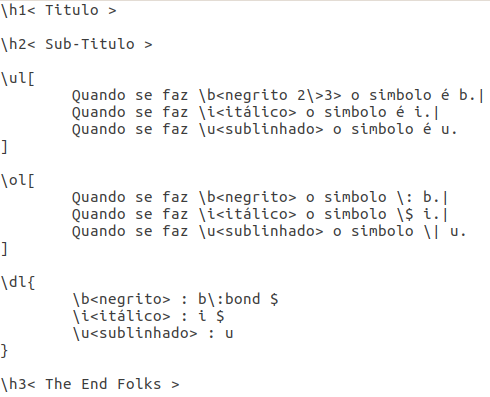
\includegraphics[width=10cm,height= 8cm]{exemplo1.png}
\caption{Exemplo com as "tags" simplificadas}
\label{Exemplo 1}
\end{figure}
\begin{figure}[h]
\centering
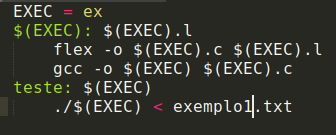
\includegraphics[width=9cm,height= 5cm]{makefile.png}
\caption{Ficheiro makefile}
\label{makefile}
\end{figure}
\begin{figure}[h]
\centering
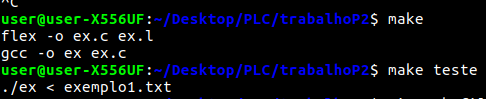
\includegraphics[width=15cm,height= 3cm]{terminal.png}
\caption{Terminal}
\label{Terminal}
\end{figure}
\begin{figure}[h]
\centering
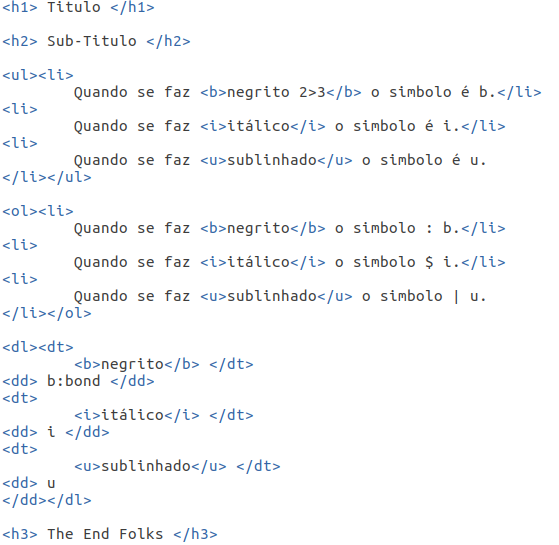
\includegraphics[width=12cm,height= 10cm]{exemplo1html.png}
\caption{Exemplo 1 depois do pré-processador}
\label{Ficheiro em HTML}
\end{figure}
\begin{figure}[h]
\centering
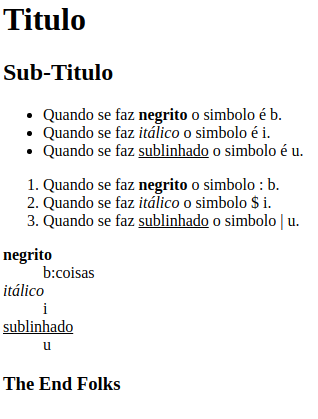
\includegraphics[width=9cm,height= 9cm]{HTML.png}
\caption{Exemplo HTML}
\label{HTML}
\end{figure}


\chapter{Código do Pré-Processador}

\begin{code}
%{
/* Declaracoes C diversas */
#include <stdio.h>
#include <stdlib.h>
#include <string.h>
#define Max 128

int n = 0;
char st[Max][32] = {0};
FILE* f;

void insere(char *id ){
	int i;
	for (i=0; id[i]!='\0'; i++){
		st[n][i] = id[i];
	}
	st[n][i-1] = '\0';
}

%}

%option noyywrap

%x TEXT SIMB

%%

			{BEGIN TEXT;}

<TEXT>{
	">"		{fprintf(f, "</%s>", st[--n] );}
	"]"		{fprintf(f, "</li></%s>", st[--n]);}
	"|"		{fprintf(f,"</li>\n<li>");}
	"}"		{fprintf(f, "</dd></%s>", st[--n]);}
	"$"		{fprintf(f,"</dd>\n<dt>");}
	":"		{fprintf(f,"</dt>\n<dd>");}
	"\\"		{BEGIN SIMB; strcpy(st[n],"");}
	.|\n		{fprintf(f, "%s", yytext );}
}

<SIMB>{
	[bui]<|h[1-6]< 	{BEGIN TEXT; insere(yytext); fprintf(f, "<%s>", st[n++] ); }
	[ou]l\[ 	{BEGIN TEXT; insere(yytext); fprintf(f, "<%s><li>", st[n++] );}
	dl\{ 		{BEGIN TEXT; insere(yytext); fprintf(f, "<%s><dt>", st[n++] );}
	.|\n		{BEGIN TEXT; fprintf(f,"%s",yytext);}
}

%%

int main(){
	f=fopen("ex.html", "w");
	yylex(); 
	fclose(f);
	return 0; 
}


\end{code}


\end{document}
